\documentclass[a4paper,12pt]{article}
\setlength{\parskip}{0.5pt}%
\setlength{\parindent}{20pt}%

%preamble: style and/or packages
\author{Michele Magni}
\title{PhD research proposal}
\date{January 2023}

%\usepackage{package}

\usepackage{hyperref}
\usepackage{titlesec}
\setcounter{secnumdepth}{3}
\usepackage{enumitem}
\usepackage{varwidth}
\usepackage{tasks}

\usepackage{graphicx}
\usepackage{siunitx}

%colors, boxes
\usepackage[dvipsnames]{xcolor}
\usepackage[most]{tcolorbox}
\tcbuselibrary{fitting}

\definecolor{columbiablue}{rgb}{0.61, 0.87, 1.0}
\definecolor{mossgreen}{rgb}{0.68, 0.87, 0.68}

\usepackage[super,sort&compress,comma]{natbib}
\bibliographystyle{naturemag}

%indent first line
\usepackage{indentfirst}
\setlength{\parindent}{30pt}

%captions
\usepackage[font=footnotesize,labelfont={bf,it}, textfont=it]{caption}
\usepackage[labelsep=period]{caption}

%landscape pages
\usepackage{pdflscape}
\usepackage{fancyhdr} 

%page number at bottom in landscape 
\fancypagestyle{mylandscape}{
\fancyhf{} %Clears the header/footer
\fancyfoot{% Footer
\makebox[\textwidth][r]{% Right
  \rlap{\hspace{.75cm}% Push out of margin by \footskip
    \smash{% Remove vertical height
      \raisebox{4.87in}{% Raise vertically
        \rotatebox{90}{\thepage}}}}}}% Rotate counter-clockwise
\renewcommand{\headrulewidth}{0pt}% No header rule
\renewcommand{\footrulewidth}{0pt}% No footer rule
}

%temporarily disable superscript
\DeclareRobustCommand*{\citen}[1]{%
  \begingroup
    \romannumeral-`\x % remove space at the beginning of \setcitestyle
    \setcitestyle{numbers}%
    \cite{#1}%
  \endgroup   
}


\begin{document}
	
	% cover page
	\begin{center}
	\thispagestyle{empty}
		\begin{LARGE}
		Title  \\[1 cm] \vfill
		\end{LARGE}
			
			
		\begin{Large}
			PhD research proposal \\ [1 cm]\vfill
			Author \\
			\href{mailto:<email>}{$<$email$>$} \\[1 cm]\vfill
			
			
			Month Year\\[1 cm]\vfill
			
			1st supervisor: $<$1st supervisor$>$ \\ 
			2nd supervisor: $<$2nd supervisor$>$ \\[1 cm]\vfill
			
			Department of $<$Department$>$ \\
			Faculty of $<$Faculty$>$ \\
            %choose between bnw or rgb logo
			\centerline{
			
\includegraphics[trim={0cm 1cm 2.1cm 0.5cm},clip]{../figures/UU_logo_2021_NL_RGB.jpg}
			}
			
		\end{Large}
	\end{center}
	
	% document begins
	\newpage
	%%table of contents 
	{\setlength\parskip{\fill}
		\tableofcontents
	}

    %you can start a new page anytime with \newpage
	\newpage
	
	%Abstract
	\section*{Abstract}
	\addcontentsline{toc}{section}{\protect\numberline{}Abstract}
		
	%%Introduction
    \newpage
	\section{Introduction}
 
	\subsection{Background}

    \subsubsection{An additional subsection}

    The most cited paper \citep{lowry1951protein}.
    
    You can reference a figure like this (fig.~\ref{fig:mandelbrot}). Uploadgit your own figures in the /figures/ folder.
    
    %figure template
    \begin{figure}[ht]
    \centerline{
    
\includegraphics[scale=1.2]{../figures/mandelbrot.jpg}
    }
    \caption{A caption \citep{mandelbrot1982fractal} or non-superscripted reference [\citen{mandelbrot1982fractal}]}
    \label{fig:mandelbrot}
    \end{figure}

    \newpage
	\subsection{State of the art}

    %make a list
    \begin{enumerate}
        \item 
        First item;
        \item 
        Second item;
        \item 
        Third item.
    \end{enumerate}

	\subsection{Knowledge gaps}	

     \begin{itemize}
        \item 
        First item;
        \item 
        Second item;
        \item 
        Third item. 
 	\end{itemize}


    %Add extra space 
    \vspace*{5mm}

    %Objective and research questions
    \newpage
    \section{Objective and research questions}
    
\begin{tcolorbox}[minipage,colback=Goldenrod,arc=0pt,outer arc=0pt]
\centering
\textbf{An overarching objective.}
\end{tcolorbox}

    \textbf{RQ 1.}	\emph{First research question?}\\
    
    \textbf{RQ 2.}	\emph{Second research question?}\\
    
    \textbf{RQ 3.}	\emph{Et cetera...}\\

    %Methods
    \newpage
    \section{Methods}
	\subsection{Methods tackling the first research question}
	
	\vspace*{10mm}
	
\begin{tcolorbox}[minipage,colback=columbiablue,arc=10pt,outer arc=10pt]
\centering
\textbf{RQ 1.}	\emph{First research question}
\end{tcolorbox}

    \vspace*{10mm}

    
    \noindent \textbf{a. Methodology}\\ [0.1 cm]

    \textbf{i. First step}
    
    \textbf{ii. Second step} 	
    \vspace*{5mm}
     
  %example of equation
  An equation (eq. \ref{eq:euler}):
  \begin{equation} \label{eq:euler}
  e^{ \pm i\theta } = \cos \theta \pm i\sin \theta
  \end{equation}
  
    \textbf{iii. Third step}
	\vspace*{5mm}
	
	
	\noindent \textbf{b. Novelty}\\ [0.1 cm] 
	    
\begin{tcolorbox}[minipage,colback=mossgreen,arc=10pt,outer arc=10pt]
\centering
\textbf{Paper 1. \emph{First paper}}
\end{tcolorbox}
    
    \vspace*{5mm}
    
    \noindent \textbf{c. Risks and feasibility}\\ [0.1 cm] 

    \noindent \textbf{d. Outcomes} \vspace*{5mm}

\textbf{Outcome 1.1.} Outcome 1.1\\

\textbf{Outcome 1.2.} Outcome 1.2.


    
    % you can find the template for this gantt chart in /figures/gantt_template.pptx, convert it to pdf and then to png to upload it on the document

    %example of a temporarily horizontal page
    \newpage
 	\begin{landscape}
	\thispagestyle{mylandscape}
	\vspace*{-3cm}
	\section{Timetable} 
    \begin{figure}[!htb]\vspace*{-0.4cm}
    \centerline{
    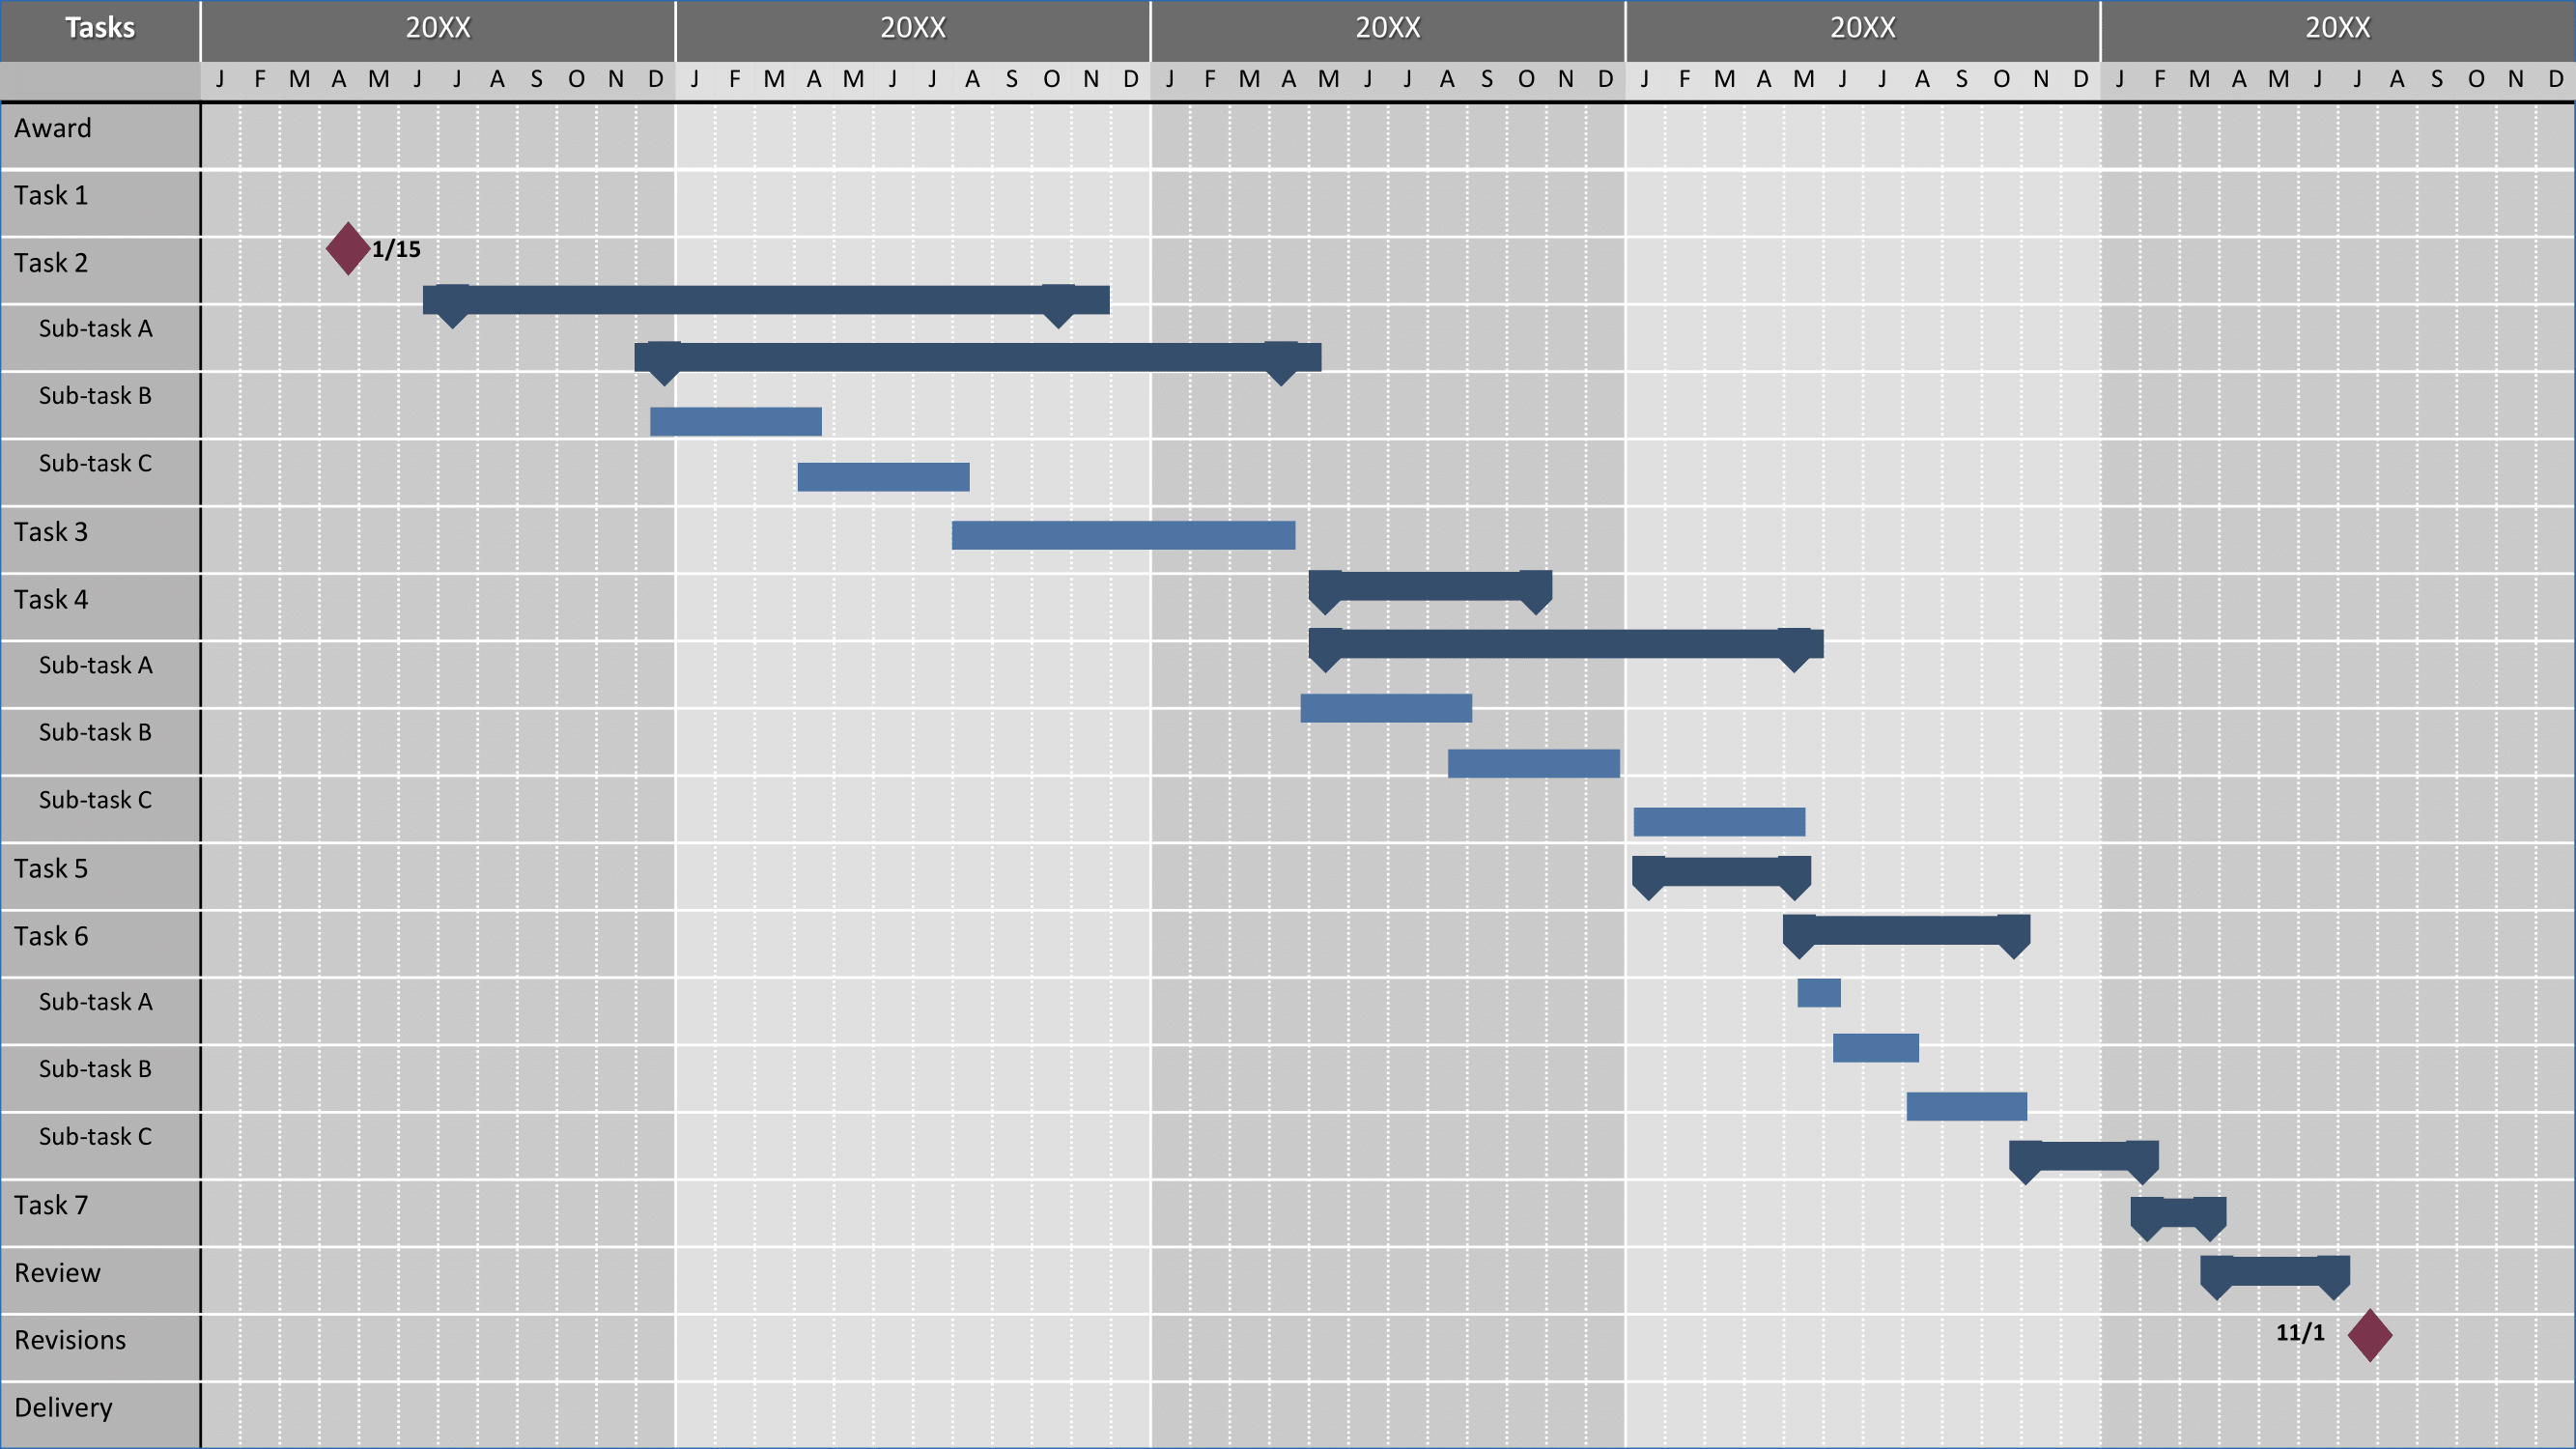
\includegraphics[scale=0.67]{../figures/gantt_template.png}
    }
    \caption{Gantt chart of the PhD project.}
    \label{fig:gantt}
    \end{figure}
    \end{landscape}
    

 		
	\newpage
	\section{Collaborations}
	\vspace*{1 cm}
    \noindent \textbf{University - Department}\\
    
    \noindent University address\\

\textbf{Theme}

    Person 1 - \href{mailto:<email>}{$<$email$>$} \\ \vspace*{-5.5mm}
    
    Person 2 – \href{mailto:<email>}{$<$email$>$} \\

\textbf{Theme 2}

    Person 1 - \href{mailto:<email>}{$<$email$>$} \\ \vspace*{-5.5mm}

    Person 2 – \href{mailto:<email>}{$<$email$>$} \\\\ 
   
    
	\section{Data management plan}
	
	\newpage
	% references
	\addcontentsline{toc}{section}{References}
	\bibliography{references.bib}
	
\end{document}